\documentclass[12pt, a4paper]{article}

\usepackage{comment}
\usepackage{ragged2e}
\usepackage{amsmath}
\usepackage{dcolumn}
\usepackage{booktabs}
\usepackage{pdflscape}
\usepackage{graphicx}
\usepackage{placeins}
\usepackage{dcolumn}
\usepackage{xcolor}
\usepackage{booktabs}
\linespread{1.5}
\usepackage{subcaption}
\usepackage{amsmath}
\usepackage{hyperref}
\usepackage{multirow}
\usepackage{tikz}
\usepackage[title]{appendix}
\usetikzlibrary{decorations.pathreplacing}
\usepackage{booktabs}
\usepackage{tabularx}
\usepackage{datatool}
\hypersetup{
	colorlinks=false,
	linkcolor=black,
	filecolor=black,      
	urlcolor=black,
	citecolor = blue
}

\usepackage{natbib}
\usepackage{xepersian}
\settextfont{XB Niloofar}
\setdigitfont{XB Zar}
\newcommand{\paren}[1]{\scaleleftright[3cm]{\text{)}}{#1}{\text{(}}}
\def\sym#1{\ifmmode^{#1}\else\(^{#1}\)\fi}

\title{مالکان نهایی و هم‌زمانی بازده شرکت با بازار}
%\subtitle{}
\author{
	مرتضی آقاجان‌زاده
	 \sym{*} 
	\qquad 
	مهدی حیدری 
	\sym{*} 
	 \\
	\sym{*} 
	\footnotesize  موسسه مطالعات پیشرفته تهران (تیاس) - دانشگاه خاتم
}

\date{
تیر 1400}




\begin{document}

\maketitle

\section{مقدمه}
\section{پیشینه پژوهش}
\section{روش‌شنای پژوهش}
\subsection{هم‌زمانی بازده شرکت}
معولا در ادبیات هم‌زمانی بازده شرکت را با ضریب تعیین برآورد خطی بازده شرکت بر روی بازده بازار و صنعت شرکت محاسبه می‌کنند. هر آنچه یک شرکت دارای ضریب تعیین بالاتری باشد، بازده شرکت با بازده بازار و یا صعنت هم زمانی بالاتری دارد. 
با توجه به مقاله 
پیتروسکی و رولستون (2004)
%\lr{\cite{piotroski2004influence} }
به منظور بدست آوردن هم زمانی قیمت سهام، معادله زیر را برای هر شرکت به صورت سالانه برازش می‌کنیم:
	\begin{equation}\label{e1}
		RET_{i,w} = \alpha + \beta_1 MKRET_{w}+ \beta_2 MKRET_{w-1}  + \beta_3 INDRET_{i,w} + \beta_4 INDRET_{i,w-1} 
	\end{equation}
	که در این معادله 
	\lr{$ RET_{i,w} $}
	بازده هفتگی شرکت i در هفته w، 
	\lr{$ MKRET_{w} $}
	بازده بازار برای هفته w و
	\lr{$ INDRET_{i,w} $}
	بازه صنعت شرکت در هفته w می‌باشد که بازده شرکت مورد بررسی از آن کم شده‌است. 
	
	ضریب تعیین بدست آمده از برازش فوق عددیدر بازه یک و منفی یک می‌باشد به همین علت نمی‌توانیم از آن به صورت مستقیم در برآورد‌های آینده استفاده کنیم. به همین منظور از تبدیل لاجستیک استفاده می‌کنیم. در نتیجه متغیر اصلی هم‌زمانی بازده شرکت برابر است با 	
	\begin{equation}
		SYNCH_{i,t} = log(\frac{R^2_{i,t}}{1-R^2_{i,t}})
	\end{equation}
که در این عبارت $  R^2_{i,t}$ ضریب تعیین بدست آمده از برازش معادله 
\ref{e1}
برای شرکت
 \lr{i}
  و در سال
 \lr{ t}
  می‌باشد. در شکل
  \ref{fig:synchtimeseries} 
  سری زمانی هم‌زمانی بازده برای تمامی شرکت‌های حاضر در بازار رسم شده‌است.
  
  
  \begin{figure}[htbp]
  	\centering
  	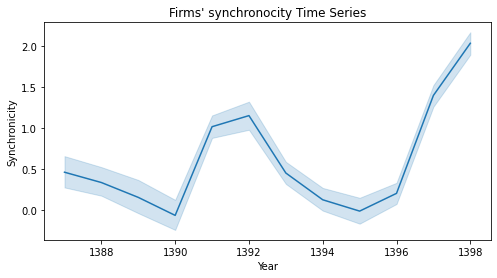
\includegraphics[width=0.85\linewidth]{SYNCHtimeSeries}
  	\caption{سری زمانی متوسط هم‌زمانی بازده شرکت‌ها }
  	\label{fig:synchtimeseries}
  \end{figure}
  
  پس از محاسبه هم‌زمانی بازده شرکت‌ها تاثیر اختلاف حق رای و حق جریان مالی شرکت‌ بر روی هم‌زمانی بازده را با برازش مدل زیر بررسی می‌کنیم:
  \begin{equation}\label{e2}
  	\begin{split}
  		\text{SYNCH}_{i,t} =&  \beta_0 + \beta_1 \text{Excess}_{i,t} + \beta_2 \text{UCF}_{i,t} \\
  		& + \sum_{k} \beta_k \text{Control}_{i,t}^k + \text{IndustryDummies} + \text{YearDummies} + \varepsilon_{i,t}
  	\end{split}
  \end{equation}
در مدل فوق عبارات i و t به ترتیب شرکت و سال را نمایندگی می‌کنند. در این مدل منظور از 
$ \text{Excess} $
پراکسی از اختلاف مالکیت و حق جریان مالی است که در چهار حالت تعریف می‌شود که عبارتند از اختلاف حق کنترل از جریان مالی  که با میزان حق رای اسکیل شده است که با 
$ \text{Excess} $
 نشان می‌دهیم.
($ \text{Excess} = (\text{cr} - \text{cfr})/\text{cr}$)  
حالت دوم این متغیر میزان اختلاف حق کنترل از حق جریان مالی می‌باشد که با 
$ \text{ExcessDiff} $
نشان داده می‌شود. دو حالت دیگر نیز دو متغیر مجازی است که چنانچه این اختلاف مثبت باشد مقدار یک به خود می‌گیرد و در غیر این صورت برابر صفر است 
 ($ \text{ExcessDummy} $)
و یا چنانچه مقدار این اختلاف از میانه این متغیر در نمونه بیشتر باشد برابر یک می‌شود و در غیر این صورت برابر صفر است.
 ($ \text{ExcessHigh} $)
$ \text{UCF} $ 
نیز حق جریان مالی مالک نهایی شرکت است. 

با توجه به تاثیر ویژگی‌های شرکت بر روی هم‌زمانی بازده شرکت، نیاز است تا ویژگی‌های شرکت نیز کنترل شود. از این روز با توجه به ادبیات از متغیر‌های نوسان بازده سهام، نقدشوندگی و اندازه استفاده شده‌است. 
در مدل فوق علاوه بر استفاده از اثر‌های ثابت سال و صنعت از کنترل شرکت نیز استفاده شده است. مشخصات آماری متغیر‌های کنترل و وابسته در جدول 
\ref{Controlsummary}
نشان داده شده‌است.

  
  
		\begin{table}[htbp]
  	\centering
  	\caption{خلاصه آماری متغیر‌های وابسته و کنترل}
  	\label{tab:Controlsummary}	
  	\begin{LTR}
  	\resizebox{0.75\textwidth}{!}{
  		\input{Controlsummary.tex}
  	}
  \end{LTR}
  	

    \end{table}




  
  
\section{یافته‌های پژوهش}


	




\lr{				\begin{table}[htbp]
	\centering
	\resizebox{0.75\textwidth}{!}{
		{
\def\sym#1{\ifmmode^{#1}\else\(^{#1}\)\fi}
\begin{tabular}{l*{8}{c}}
\hline\hline
                    &\multicolumn{8}{c}{Synchronicity}                                                                                                                                              \\\cmidrule(lr){2-9}
                    &\multicolumn{1}{c}{(1)}         &\multicolumn{1}{c}{(2)}         &\multicolumn{1}{c}{(3)}         &\multicolumn{1}{c}{(4)}         &\multicolumn{1}{c}{(5)}         &\multicolumn{1}{c}{(6)}         &\multicolumn{1}{c}{(7)}         &\multicolumn{1}{c}{(8)}         \\
\hline
Excess              &                     &      -0.899\sym{**} &      -0.557\sym{*}  &                     &                     &                     &                     &                     \\
                    &                     &     [-3.22]         &     [-2.10]         &                     &                     &                     &                     &                     \\
[1em]
ExcessDiff          &                     &                     &                     &      -0.512         &                     &                     &                     &                     \\
                    &                     &                     &                     &     [-1.61]         &                     &                     &                     &                     \\
[1em]
ExcessDummy         &                     &                     &                     &                     &     -0.0900         &                     &                     &                     \\
                    &                     &                     &                     &                     &     [-0.66]         &                     &                     &                     \\
[1em]
ExcessHigh          &                     &                     &                     &                     &                     &      -0.175         &                     &                     \\
                    &                     &                     &                     &                     &                     &     [-1.34]         &                     &                     \\
[1em]
position            &                     &                     &                     &                     &                     &                     &     -0.0959\sym{*}  &                     \\
                    &                     &                     &                     &                     &                     &                     &     [-2.53]         &                     \\
[1em]
centrality          &                     &                     &                     &                     &                     &                     &                     &       1.159\sym{**} \\
                    &                     &                     &                     &                     &                     &                     &                     &      [2.83]         \\
[1em]
cfr                 &                     &      -0.421         &      -0.173         &      0.0838         &       0.244         &       0.102         &       0.119         &       0.336         \\
                    &                     &     [-1.17]         &     [-0.53]         &      [0.31]         &      [0.96]         &      [0.38]         &      [0.50]         &      [1.53]         \\
[1em]
volatility          &    -0.00453         &                     &     -0.0184         &     -0.0168         &     -0.0137         &     -0.0171         &     -0.0182         &     -0.0135         \\
                    &     [-0.27]         &                     &     [-0.95]         &     [-0.87]         &     [-0.69]         &     [-0.86]         &     [-0.92]         &     [-0.69]         \\
[1em]
Liquidity           &      -0.206\sym{***}&                     &      -0.191\sym{***}&      -0.192\sym{***}&      -0.196\sym{***}&      -0.195\sym{***}&      -0.195\sym{***}&      -0.190\sym{***}\\
                    &     [-9.33]         &                     &     [-6.17]         &     [-6.29]         &     [-6.29]         &     [-6.31]         &     [-6.30]         &     [-5.91]         \\
[1em]
Size                &     -0.0873\sym{**} &                     &     -0.0952\sym{*}  &     -0.0917\sym{*}  &     -0.0853\sym{*}  &     -0.0879\sym{*}  &      -0.101\sym{*}  &     -0.0789         \\
                    &     [-3.03]         &                     &     [-2.17]         &     [-2.09]         &     [-2.01]         &     [-2.06]         &     [-2.25]         &     [-1.88]         \\
[1em]
leverage            &      -0.104         &                     &      -0.281\sym{*}  &      -0.291\sym{*}  &      -0.286\sym{*}  &      -0.273\sym{*}  &      -0.334\sym{**} &      -0.199         \\
                    &     [-1.79]         &                     &     [-2.38]         &     [-2.50]         &     [-2.47]         &     [-2.35]         &     [-2.77]         &     [-1.61]         \\
[1em]
 $ \ln(NIND) $      &      -0.138         &                     &      -0.522         &      -0.526         &      -0.567         &      -0.585         &      -0.602         &      -0.396         \\
                    &     [-0.36]         &                     &     [-0.55]         &     [-0.55]         &     [-0.59]         &     [-0.61]         &     [-0.64]         &     [-0.41]         \\
\hline
Industry Dummy      &         Yes         &         Yes         &         Yes         &         Yes         &         Yes         &         Yes         &         Yes         &         Yes         \\
Year Dummy          &         Yes         &         Yes         &         Yes         &         Yes         &         Yes         &         Yes         &         Yes         &         Yes         \\
Observations        &        2550         &        1116         &         978         &         978         &         978         &         978         &         978         &         941         \\
$ R^2 $             &       0.357         &       0.444         &       0.479         &       0.478         &       0.477         &       0.477         &       0.479         &       0.493         \\
\hline\hline
\multicolumn{9}{l}{\footnotesize \textit{t} statistics in brackets}\\
\multicolumn{9}{l}{\footnotesize \sym{*} \(p<0.05\), \sym{**} \(p<0.01\), \sym{***} \(p<0.001\)}\\
\end{tabular}
}

		\label{tab:synchronicityt4}	
	}
\end{table}}



 
\lr{	\begin{table}[htbp]
		\centering
		\resizebox{0.75\textwidth}{!}{
			{
\def\sym#1{\ifmmode^{#1}\else\(^{#1}\)\fi}
\begin{tabular}{l*{8}{c}}
\hline\hline
                    &\multicolumn{8}{c}{Synchronicity}                                                                                                                                              \\\cmidrule(lr){2-9}
                    &\multicolumn{1}{c}{(1)}         &\multicolumn{1}{c}{(2)}         &\multicolumn{1}{c}{(3)}         &\multicolumn{1}{c}{(4)}         &\multicolumn{1}{c}{(5)}         &\multicolumn{1}{c}{(6)}         &\multicolumn{1}{c}{(7)}         &\multicolumn{1}{c}{(8)}         \\
\hline
Excess              &                     &      -0.894\sym{**} &      -0.486         &                     &                     &                     &                     &                     \\
                    &                     &     [-4.64]         &     [-2.50]         &                     &                     &                     &                     &                     \\
[1em]
ExcessDiff          &                     &                     &                     &      -0.492         &                     &                     &                     &                     \\
                    &                     &                     &                     &     [-2.05]         &                     &                     &                     &                     \\
[1em]
ExcessDummy         &                     &                     &                     &                     &     -0.0777         &                     &                     &                     \\
                    &                     &                     &                     &                     &     [-1.55]         &                     &                     &                     \\
[1em]
ExcessHigh          &                     &                     &                     &                     &                     &      -0.191         &                     &                     \\
                    &                     &                     &                     &                     &                     &     [-1.73]         &                     &                     \\
[1em]
position            &                     &                     &                     &                     &                     &                     &     -0.0575         &                     \\
                    &                     &                     &                     &                     &                     &                     &     [-2.08]         &                     \\
[1em]
centrality          &                     &                     &                     &                     &                     &                     &                     &       1.497\sym{***}\\
                    &                     &                     &                     &                     &                     &                     &                     &      [7.48]         \\
[1em]
cfr                 &                     &      -0.468         &      -0.269         &     -0.0738         &      0.0783         &      -0.104         &      0.0265         &       0.169         \\
                    &                     &     [-1.58]         &     [-0.79]         &     [-0.25]         &      [0.31]         &     [-0.31]         &      [0.14]         &      [0.81]         \\
[1em]
volatility          &       0.489\sym{**} &                     &       1.654\sym{*}  &       1.616\sym{*}  &       1.615\sym{*}  &       1.686\sym{*}  &       1.657\sym{*}  &       1.580\sym{*}  \\
                    &      [6.17]         &                     &      [2.77]         &      [2.79]         &      [2.79]         &      [2.79]         &      [2.75]         &      [2.83]         \\
[1em]
Liquidity           &      -0.219\sym{***}&                     &      -0.242\sym{***}&      -0.243\sym{***}&      -0.248\sym{***}&      -0.239\sym{***}&      -0.246\sym{***}&      -0.220\sym{***}\\
                    &    [-12.25]         &                     &    [-20.05]         &    [-19.89]         &    [-18.27]         &    [-16.05]         &    [-16.07]         &    [-10.85]         \\
[1em]
Size                &     -0.0910\sym{**} &                     &      -0.126\sym{**} &      -0.125\sym{**} &      -0.115\sym{*}  &      -0.117\sym{*}  &      -0.122\sym{*}  &      -0.101\sym{*}  \\
                    &     [-4.42]         &                     &     [-4.37]         &     [-4.46]         &     [-3.54]         &     [-3.70]         &     [-3.37]         &     [-2.92]         \\
[1em]
leverage            &     -0.0837         &                     &     -0.0894         &     -0.0997         &     -0.0969         &     -0.0835         &      -0.136         &      0.0254         \\
                    &     [-2.31]         &                     &     [-0.52]         &     [-0.59]         &     [-0.58]         &     [-0.47]         &     [-0.82]         &      [0.13]         \\
[1em]
 $ \ln(NIND) $      &      -0.735\sym{**} &                     &      -0.368         &      -0.376         &      -0.593         &      -0.434         &      -0.463         &      -0.398         \\
                    &     [-6.34]         &                     &     [-1.61]         &     [-1.44]         &     [-1.86]         &     [-1.62]         &     [-1.91]         &     [-1.34]         \\
\hline
Industry Dummy      &         Yes         &         Yes         &         Yes         &         Yes         &         Yes         &         Yes         &         Yes         &         Yes         \\
Year Dummy          &          No         &          No         &          No         &          No         &          No         &          No         &          No         &          No         \\
Observations        &        2550         &        1116         &         978         &         978         &         978         &         978         &         978         &         941         \\
$ R^2 $             &       0.327         &       0.462         &       0.547         &       0.547         &       0.544         &       0.546         &       0.550         &       0.568         \\
\hline\hline
\multicolumn{9}{l}{\footnotesize \textit{t} statistics in brackets}\\
\multicolumn{9}{l}{\footnotesize \sym{*} \(p<0.05\), \sym{**} \(p<0.01\), \sym{***} \(p<0.001\)}\\
\end{tabular}
}

			\label{tab:synchronicityt5}	
		}
	\end{table}}



\section{نتیجه‌گیری و پیشنهاد‌ها}

\begin{LTR}		
	\bibliographystyle{apalike}
	\bibliography{Ref}
\end{LTR}
\end{document}